% Scheduling Policies in AsyncFlow: why coupled AI-HPC workflows need them
% rust results: design/rust-experiments.md and results/; second campaign: design/rust-experiments-2.md and results/r2/; third (two nodes, diagnostics C and D): design/rust-experiments-3.md and results/r3/; fourth (switch e): design/rust-experiments-4.md and results/r4/; fifth (PSC Bridges-2, 2 and 4 nodes): design/bridges2-experiments.md and results/b2/; sixth (NERSC Perlmutter, 2 and 4 nodes, kit policy-order): the experiment kit at 2f8a8bc, copied to results/pm/charts/. Build: latexmk -lualatex -outdir=build scheduling-policies.tex
\documentclass[aspectratio=169, 10pt, t]{beamer}
\usetheme{lecture}

\usepackage{listings}
\graphicspath{{results/}}
\lstdefinestyle{py}{language=Python,
  basicstyle=\ttfamily\fontsize{7}{8.8}\selectfont,
  keywordstyle=\color{titleink}\bfseries,
  commentstyle=\color{labelgray}\itshape,
  stringstyle=\color{bodyink},
  backgroundcolor=\color{boxgray}, frame=single, rulecolor=\color{boxline},
  framesep=4pt, xleftmargin=4pt, xrightmargin=4pt, aboveskip=2pt, belowskip=4pt,
  showstringspaces=false, columns=fullflexible, keepspaces=true, upquote=true,
  morekeywords={async, await}}
\lstset{style=py}

% A dashed box standing in for a result still to be measured
\newcommand{\pending}[2]{%
  \begin{center}\begin{tikzpicture}
    \node[box, dashed, minimum width=#1, minimum height=2.6cm, fill=boxgray,
          font=\fontsize{8}{9.6}\selectfont, text=labelgray] {#2};
  \end{tikzpicture}\end{center}}

\title{Scheduling Policies in AsyncFlow}
\subtitle{Why coupled AI--HPC workflows need them, and what they buy\\{}[Venue], [Date]}
\author{Matteo Turilli}
\date{}

\begin{document}

\begin{frame}[plain]
  \titlepage
\end{frame}

\begin{frame}{What I Am Showing Today}
\begin{itemize}
  \item Coupled AI--HPC workflows need decisions that the backend cannot make on its own.
  \item What we built: a tickless engine, opt-in ordering policies and resource-aware admission, plus a RHAPSODY change so Dragon places tasks where AsyncFlow decides.
  \item The evidence so far: microbenchmarks, a simulated backend and a simulation of IMPRESS on 8 Delta nodes.
  \item Experiments on rust, with real Dragon and real GPUs: what holds, and what Dragon changes.
  \item The Dragon changes that let Dragon and AsyncFlow cooperate, and what they mean for AsyncFlow's design.
  \item One Dragon runtime over two nodes: where placement pays, and what it costs.
  \item Two and four nodes on PSC Bridges-2: the policies hold, and a multi-node runtime costs throughput.
  \item Two and four nodes on NERSC Perlmutter with stock Dragon 0.15.0: the policies hold on \code{Batch} and on a native backend.
  \item What we ask Dragon; what is proven, what is not yet, and what comes next.
\end{itemize}
\end{frame}

\divider{A. The Problem}

\begin{frame}{Coupled AI--HPC Workflows Mix Very Different Work}
\begin{itemize}
  \item \textbf{Hours and milliseconds.} Simulations run for hours, while a learner or selection step needs seconds (ROSE active learning).
  \item \textbf{Shared GPUs.} Many pipelines share each GPU, and memory, not the device count, sets the limit (IMPRESS runs 8 pipelines per GPU).
  \item \textbf{Adaptive loops.} The next batch depends on results that may still be waiting in a queue.
  \item \textbf{Services beside tasks.} Inference servers run next to the tasks that call them (MATEY, vLLM).
\end{itemize}
\vfill
\begin{center}
  \begin{tikzpicture}
    \node[bluebox, text width=12.5cm, font=\fontsize{10}{12}\selectfont, inner sep=6pt]
      {Today AsyncFlow hands every ready task to the backend at once.\\The backend's queue decides what runs next, and where.};
  \end{tikzpicture}
\end{center}
\vfill
\end{frame}

\begin{frame}{The Backend and the Workflow Each Know Half}
\begin{lecturetable}{\footnotesize}
\begin{tabular}{|B{2.6cm}|L{5.3cm}|L{6.0cm}|}
\hline
\head Layer & Knows & Does not know \\ \hline
Backend (Dragon, a thread pool) & Its workers and its queue; roughly which nodes are free & Which task unblocks a learner step; which workflow is interactive; a task's GPU memory (Dragon 0.14 counts neither GPUs nor memory) \\ \hline
AsyncFlow & The DAG, lineage, workflow scopes, declared resources, the results that come back & Without a policy, it uses none of this: a ready task is submitted at once \\ \hline
\end{tabular}
\end{lecturetable}
\vfill
\begin{center}
  {\fontsize{12}{14}\selectfont\color{titleink}A policy puts the decision where the knowledge is.}
\end{center}
\vfill
\end{frame}

\divider{B. What We Built}

\begin{frame}{Four Pieces, Stacked as Pull Requests}
\bodysmall
\begin{itemize}
  \item Each piece is engine-internal or opt-in. Withdrawing one leaves the ones below it unchanged.
\end{itemize}
\vfill
\begin{center}
\begin{tikzpicture}[x=1cm, y=1cm]
  \node[graybox, minimum width=2.4cm, minimum height=1.1cm] (b) at (3,0) {\#100\\hot path\\(open, on main)};
  \node[bluebox, minimum width=2.4cm, minimum height=1.1cm] (c) at (6,0) {\#110\\tickless run loop\\(open, replaces \#91)};
  \node[bluebox, minimum width=2.4cm, minimum height=1.1cm] (d) at (9,0) {Ordering policies\\(branch)};
  \node[bluebox, minimum width=2.4cm, minimum height=1.1cm] (e) at (12,0) {Resource-aware\\admission (branch)};
  \foreach \u/\v in {b/c, c/d, d/e} \draw[arrow] (\u) -- (\v);
  \node[box, minimum width=3.6cm, minimum height=1.1cm] (r1) at (6,-2.3) {RHAPSODY \#105\\Dragon cancellations\\on the event loop (merged)};
  \node[box, minimum width=3.6cm, minimum height=1.1cm] (r2) at (12,-2.3) {RHAPSODY placement\\Dragon runs a task where\\AsyncFlow places it (branch)};
  \draw[arrow] (e.south) -- node[label, left] {writes a placement} (r2.north);
  \draw[arrow, dashed] (r1.north) -- node[label, right] {cancellations reported from a thread} (c.south);
  \node[caption, anchor=west] at (1.8,1.1) {AsyncFlow};
  \node[caption, anchor=west] at (1.8,-1.45) {RHAPSODY};
\end{tikzpicture}
\end{center}
\vfill
\end{frame}

\begin{frame}{Tickless Engine (\#110): No Polling, No Idle Cost}
\begin{lecturetable}{\footnotesize}
\begin{tabular}{|B{7.2cm}|L{3.0cm}|L{3.0cm}|}
\hline
\head Measure & \#100 & \#110 \\ \hline
Sequential chain, per task & 10.4 ms & 34.6 µs \\ \hline
Dependency edge, task completed from a backend thread & 19.9 ms & 2.23 ms \\ \hline
Idle CPU with 10,000 tasks in flight & 0.66\% of a core & 0.004\% \\ \hline
1,024 concurrent diamonds, 10,000 tasks in flight & 27,650 tasks/s & 41,380 tasks/s \\ \hline
Dragon: dependency edge in a chain (median) & 563 ms & 1.0 ms \\ \hline
Dragon-side cancellation, until the dependent is released & 406--708 ms & 0.1--0.2 ms \\ \hline
\end{tabular}
\end{lecturetable}
\vfill
{\fontsize{7}{8.4}\selectfont\color{labelgray}AMD EPYC 7502P, Python 3.14, one pinned core; the Dragon rows: dragonhpc 0.14.1 on one node. \#100 at 5ccf4a2 (on main, polling every 10 ms when busy, 1 s when idle), \#110 at 437a10d, 2026-10-31. Unit suite: 214 tests on Python 3.9 and 3.13.\par}
\end{frame}

\begin{frame}[fragile]{Ordering Policies Are One Argument}
\begin{lstlisting}
from radical.asyncflow import FairPolicy, WorkflowEngine

flow = await WorkflowEngine.create(
    backend=backend,
    policy=FairPolicy(64, weights={"interactive": 4}))

async with flow.workflow_scope("bulk"):
    sims = [simulate(i) for i in range(4000)]

async with flow.workflow_scope("interactive"):
    step = learn(select(*sims[:16]))   # starts ahead of the bulk
\end{lstlisting}
\bodysmall
\begin{itemize}
  \item \code{FifoPolicy(capacity)}: ready order, at most \code{capacity} tasks in flight.
  \item \code{LineagePolicy(capacity)}: started workflows finish before new ones start.
  \item \code{FairPolicy(capacity, weights)}: weighted fair share across workflow scopes.
  \item Without a policy nothing changes.
\end{itemize}
\end{frame}

\begin{frame}[fragile]{A Policy Is Four Operations}
\begin{lstlisting}
class Policy(Protocol):
    def enqueue(self, uid: str, desc: dict) -> None: ...
    def dispatch(self) -> list[dict]: ...
    def release(self, uid: str, ran: bool = True,
                observed: dict | None = None) -> bool: ...
    def runnable(self) -> bool: ...
\end{lstlisting}
\bodysmall
\begin{itemize}
  \item \code{enqueue}: a task is ready. Raising rejects it, and the engine fails the task.
  \item \code{dispatch}: the tasks to submit now.
  \item \code{release}: a task left the backend, with the resource use the backend observed.
  \item \code{runnable}: is there anything to dispatch now?
  \item Blocks and services bypass the policy. The engine calls it on its event-loop thread, so a policy needs no locking.
\end{itemize}
\end{frame}

\begin{frame}[fragile]{Resource-Aware Admission: Tasks Declare What They Need}
\begin{lstlisting}
from radical.asyncflow import MemoryModel, NodeShape, Pool, ResourcePolicy

node = NodeShape(cpus=64, gpus=4, host_mem=256, gpu_mem=40)   # GiB
policy = ResourcePolicy(Pool([node] * 8, mode="node"), memory=MemoryModel())
flow = await WorkflowEngine.create(backend=backend, policy=policy)

fold(seq, task_description={"resources": {"gpus": 0.25, "gpu_mem": 9}})
# admitted when a GPU has a quarter and 9 GiB free, then
# task["placement"] = {"node": 3, "host": "gpu003", "gpus": [1]}
\end{lstlisting}
\bodysmall
\begin{itemize}
  \item \textbf{aggregate}: the demand fits the pool's free totals.
  \item \textbf{node}: the demand fits one node, and a GPU share one GPU. AsyncFlow picks them and RHAPSODY's Dragon backend runs the task there.
  \item Memory is learned from the peaks a backend reports. A demand that can never fit fails at once.
\end{itemize}
\end{frame}

\divider{C. Evidence So Far}

\begin{frame}{Ordering: Short Steps Stop Waiting Behind Bulk Work}
\begin{lecturetable}{\footnotesize}
\begin{tabular}{|B{6.2cm}|L{1.7cm}|L{1.7cm}|L{1.7cm}|L{1.7cm}|}
\hline
\head & None & FIFO & Lineage & Fair \\ \hline
\multicolumn{5}{|l|}{\textit{4,000 bulk 5 ms tasks beside a 3-step interactive chain every 50 ms}} \\ \hline
Chain latency, p50 & 905 ms & 915 ms & 924 ms & \textbf{20 ms} \\ \hline
Bulk makespan & 1.394 s & 1.401 s & 1.417 s & 1.445 s \\ \hline
\multicolumn{5}{|l|}{\textit{512 concurrent diamond workflows, 2 ms tasks}} \\ \hline
Mean workflow completion & 0.210 s & 0.213 s & \textbf{0.138 s} & 0.203 s \\ \hline
First workflow done & 0.173 s & 0.176 s & \textbf{0.026 s} & 0.167 s \\ \hline
Workflows in progress at peak & 512 & 512 & \textbf{16} & 512 \\ \hline
\end{tabular}
\end{lecturetable}
\vfill
{\fontsize{7}{8.4}\selectfont\color{labelgray}Simulated backend with 16 workers and a FIFO queue, as ThreadPoolExecutor has (Dragon's \code{Batch} turned out not to be strictly FIFO: see E1); policy capacity 16; medians of 5 runs on one pinned core of an AMD EPYC 7502P.\par}
\end{frame}

\begin{frame}{Resources: IMPRESS on 8 Delta Nodes, Simulated}
\begin{lecturetable}{\footnotesize}
\begin{tabular}{|B{4.4cm}|L{2.3cm}|L{2.2cm}|L{2.2cm}|L{2.4cm}|}
\hline
\head Admission & CUDA OOMs & Pipelines lost & Passing folds & GPU-h per fold \\ \hline
None & 183 & 183 & 976 & 0.131 \\ \hline
Staggered start (today) & 73 & 73 & 2,216 & 0.058 \\ \hline
At most 16 tasks per node & 96 & 96 & 1,566 & 0.082 \\ \hline
Aggregate (pool totals) & 156 & 156 & 1,261 & 0.110 \\ \hline
Node, declared memory & \textbf{0} & \textbf{0} & \textbf{2,833} & \textbf{0.045} \\ \hline
Node, learned memory & 0 & 0 & 2,798 & 0.046 \\ \hline
\end{tabular}
\end{lecturetable}
\vspace{4pt}
\bodysmall
\begin{itemize}
  \item Totals that fit still overload single GPUs: Dragon picks the node, and the application picks the GPU.
  \item Node mode: no failures, 28\% more passing folds than today, 22\% fewer GPU-hours per fold.
\end{itemize}
\vfill
{\fontsize{7}{8.4}\selectfont\color{labelgray}Simulation: 256 pipelines (8 per GPU), 4 h, means of 5 seeds. The model reproduces IMPRESS's measured one-node ladder within a few percent; its model of Dragon's placement on 8 nodes is not yet checked against a real run.\par}
\end{frame}

\begin{frame}{What It Costs}
\begin{lecturetable}{\footnotesize}
\begin{tabular}{|B{6.8cm}|L{7.4cm}|}
\hline
\head Configuration & Cost \\ \hline
Policy hook, no policy set & Nothing measurable: 31.85 against 31.5--32.05 µs per task \\ \hline
Ordering policies & 1--4\% of makespan with 2--5 ms tasks \\ \hline
\code{ResourcePolicy}, aggregate & 15 µs per task \\ \hline
\code{ResourcePolicy}, node (8 nodes of 4 GPUs) & 28 µs per task \\ \hline
The engine itself, for comparison & About 31 µs per task \\ \hline
\end{tabular}
\end{lecturetable}
\vfill
\begin{itemize}
  \item Negligible for tasks that run for seconds; noticeable for millisecond tasks.
  \item Admission is not optimised yet.
\end{itemize}
\vfill
{\fontsize{7}{8.4}\selectfont\color{labelgray}AMD EPYC 7502P, Python 3.14, one pinned core; 20,000 tasks of 4 kinds waiting for the admission rows.\par}
\end{frame}

\divider{D. Experiments on rust}

\begin{frame}{Testbed: The rust Cluster}
\begin{itemize}
  \item \textbf{haskell:} 2 AMD EPYC 9755, 512 threads, 406 GB; 2 NVIDIA RTX 6000 Ada (48 GB each).
  \item \textbf{julia:} 2 AMD EPYC 9745, 512 threads, 515 GB; 1 NVIDIA RTX PRO 6000 Blackwell Server Edition.
  \item \textbf{fortran:} 2 NVIDIA RTX PRO 6000 Blackwell (95 GiB each), in partitions of its own.
  \item Slurm 24.11 on Proxmox VMs. No HSTA fabric, so Dragon runs over TCP.
  \item A user may hold at most 128 CPUs and 2 GPUs, so every run uses part of a node. Another job may share its cores.
  \item Two Dragon jobs of one user must not share a node: \code{dragon-cleanup} in one kills the other's runtime.
  \item Four campaigns, each configuration 3 times, interleaved. The first: the stock dragonhpc 0.14.1 wheel, RHAPSODY with \code{Batch}'s pool capped to the job's CPUs, and the AsyncFlow policy branches. The second added a local Dragon branch (section E); the third ran one Dragon runtime over two nodes (section F); the fourth added a fifth switch.
\end{itemize}
\end{frame}

\begin{frame}{Dragon on rust: Issue \#95 Was Oversubscription}
\bodysmall
\begin{itemize}
  \item \code{Batch} sized its worker pool from the node's 512 CPUs, not from the CPUs the job holds. On a 4-CPU job, about 280 Dragon processes shared 4 CPUs.
\end{itemize}
\begin{lecturetable}{\footnotesize}
\begin{tabular}{|B{6.0cm}|L{2.6cm}|L{2.6cm}|L{2.6cm}|}
\hline
\head 4-CPU job & One trivial task & 3-task workflow & Shutdown \\ \hline
Pool sized from 512 CPUs (stock) & 111 s & 271 s & over 5 min \\ \hline
Pool sized from the job's CPUs & 0.5 s & 2.5 s & 1.2 s \\ \hline
Patched Dragon, no workaround & 0.3 s & 2.2 s & not timed \\ \hline
\end{tabular}
\end{lecturetable}
\vspace{4pt}
\begin{itemize}
  \item The fix sizes the pool from the CPUs Dragon may use: a local Dragon branch from v0.14.1. Dragon 0.15.0 still sizes it the old way.
  \item Also checked on rust: Dragon pins a placed task to its GPU, and runs across haskell and julia over TCP.
\end{itemize}
\vfill
{\fontsize{7}{8.4}\selectfont\color{labelgray}dragonhpc 0.14.1, rhapsody-py 0.6.0, radical.asyncflow 0.6.0 on haskell; times from the scripts' own timestamps.\par}
\end{frame}

\begin{frame}{Found First: Dragon Reports Tasks in Bursts}
\bodysmall
\begin{itemize}
  \item Dragon 0.14.1's \code{Batch} launches each round of ready tasks with one \code{map\_async}, and reports the round only when all its tasks have finished. Its client also groups submissions that arrive within 5 ms.
\end{itemize}
\begin{lecturetable}{\footnotesize}
\begin{tabular}{|B{4.6cm}|L{4.2cm}|L{4.8cm}|}
\hline
\head 6 tasks of 1--6 s, submitted & Each task ended at & Reported at \\ \hline
In a tight loop & +1.0, +2.0, \dots, +6.0 s & All at +6.0 s \\ \hline
50 ms apart & +1.0, +2.0, \dots, +6.0 s & Within 0.05 s of its end \\ \hline
\end{tabular}
\end{lecturetable}
\vspace{4pt}
\begin{itemize}
  \item AsyncFlow submits the ready tasks of a round together, so a task's completion waits for the slowest task launched with it. A policy with a capacity refills its slots in waves.
  \item \code{Batch} is not strictly FIFO either: it orders ready tasks by their position in a compiled group, then by task id as text. A late submission overtakes a backlog.
  \item So E1 and E2 ran two ways: \textbf{stock}, what users get today; and \textbf{8 ms apart}, so each task lands in a round of its own. No Dragon change, but submission is capped at about 125 tasks/s: a diagnostic, not a fix.
\end{itemize}
\vfill
{\fontsize{7}{8.4}\selectfont\color{labelgray}\code{Batch} without RHAPSODY, 8 workers on haskell (job 24476). Through RHAPSODY and AsyncFlow, the same 6 tasks were all seen at +6.1 s (job 24473).\par}
\end{frame}

\begin{frame}{E1: Fair Share Keeps Chains Short on Real Dragon}
\begin{columns}[T]
\begin{column}{0.55\textwidth}
  \vspace{2pt}
  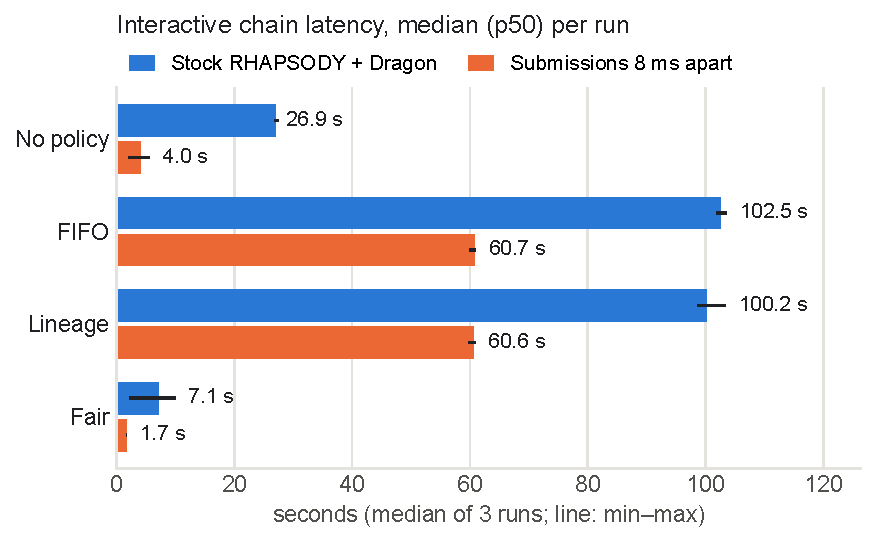
\includegraphics[width=\linewidth]{e1_chain_latency.pdf}
\end{column}
\begin{column}{0.43\textwidth}
\bodysmall
\begin{itemize}
  \item 1,000 bulk tasks of 1--5 s. Every 6 s, a chain of 3 steps of 0.5 s.
  \item \textbf{Fair:} chains take 7.1 s on stock Dragon and 1.7 s 8 ms apart, against 26.9 s and 4.0 s with no policy.
  \item The bulk pays about 1\% of makespan against FIFO, and nothing against no policy.
  \item \textbf{FIFO and Lineage are slower than no policy}: a late chain step overtakes Dragon's backlog, but not a policy's queue.
\end{itemize}
\end{column}
\end{columns}
\vfill
{\fontsize{7}{8.4}\selectfont\color{labelgray}julia, 64 CPUs, 32 \code{Batch} workers; capacity 32, Fair without weights; p50 by nearest rank over 12 chains, median of 3 runs. Simulated, Fair cut the p50 45 times; here 4 times (stock) and 2.4 times (8 ms apart). Stock Fair varies between runs: a rerun gave 2.4 s.\par}
\end{frame}

\begin{frame}{E1: Lineage Finishes Workflows Sooner}
\bodysmall
\begin{itemize}
  \item 256 diamond workflows t1 $\rightarrow$ (t2, t3) $\rightarrow$ t4 of 1 s tasks, all registered at once: 32 s of work for 32 workers.
\end{itemize}
\begin{lecturetable}{\scriptsize}
\renewcommand{\arraystretch}{1.3}
\begin{tabular}{|B{5.0cm}|L{1.9cm}|L{1.9cm}|L{1.9cm}|L{1.9cm}|}
\hline
\head & None & FIFO & Lineage & Fair \\ \hline
\multicolumn{5}{|l|}{\textit{Submissions 8 ms apart}} \\ \hline
Mean workflow completion & 26.5 s & 29.6 s & \textbf{18.4 s} & 29.6 s \\ \hline
First workflow done & 21.4 s & 25.8 s & \textbf{3.1 s} & 25.8 s \\ \hline
Workflows in progress at peak & 229 & 256 & \textbf{32} & 256 \\ \hline
\multicolumn{5}{|l|}{\textit{Stock RHAPSODY + Dragon}} \\ \hline
Mean workflow completion & 19.2 s & 30.3 s & \textbf{18.7 s} & 30.1 s \\ \hline
First workflow done & 5.3 s & 26.3 s & \textbf{3.2 s} & 26.3 s \\ \hline
Workflows in progress at peak & 64 & 256 & \textbf{32} & 256 \\ \hline
\end{tabular}
\end{lecturetable}
\vspace{4pt}
\begin{itemize}
  \item 8 ms apart, Lineage reproduces the simulation: mean completion $-$31\% (simulated $-$34\%), for +3\% makespan.
  \item On stock Dragon, no policy already behaves almost like Lineage, by an accident of the burst reports: later t2, t3 and t4 overtake the queued t1s. Lineage gains 3\%.
\end{itemize}
\vfill
{\fontsize{7}{8.4}\selectfont\color{labelgray}julia, 64 CPUs, 32 \code{Batch} workers, policy capacity 32; median of 3 runs. Makespan 33.4--35.3 s in every configuration.\par}
\end{frame}

\begin{frame}{E2: Node Mode Kept Every Pipeline on Real GPUs}
\bodysmall
\begin{itemize}
  \item haskell's 2 GPUs, 24 IMPRESS-like pipelines (12 per GPU; IMPRESS runs 8). Synthetic CUDA tasks hold an IMPRESS-like footprint, and a CUDA OOM ends its pipeline.
\end{itemize}
\begin{center}
  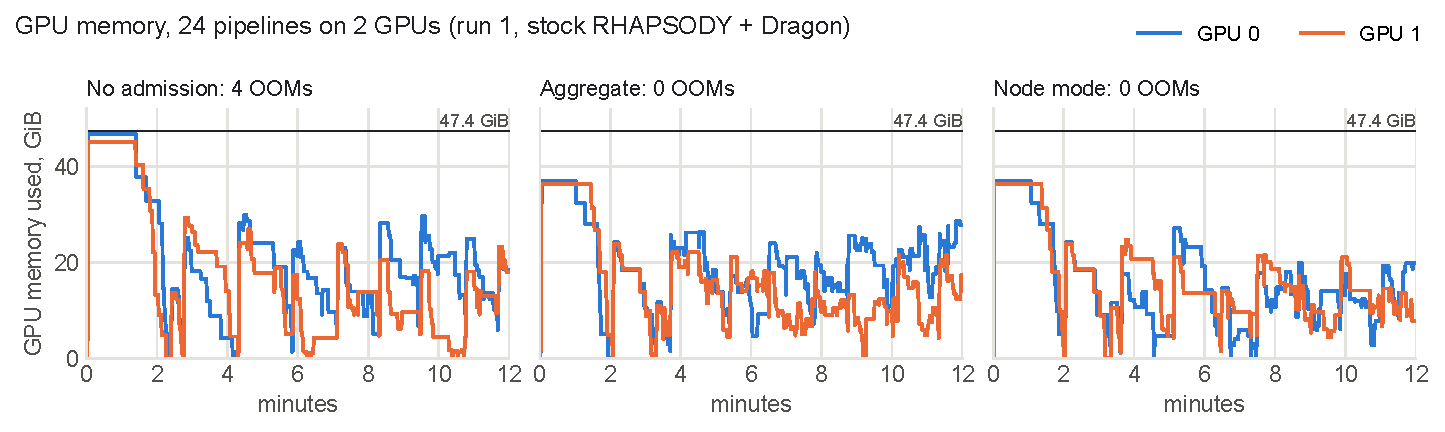
\includegraphics[width=0.88\textwidth]{e2_gpu_memory_stock.pdf}
\end{center}
\begin{itemize}
  \item \textbf{No admission:} 4--6 of 24 pipelines lost per run, 27 of 28 OOMs in the first second.
  \item \textbf{Node mode:} no OOM in 6 runs; all 1,791 tasks ran on the GPU AsyncFlow chose.
  \item \textbf{Aggregate:} one OOM in 6 runs: the application put 10 tasks on one GPU, while the totals fit.
\end{itemize}
\end{frame}

\begin{frame}{E2: Admission Did Not Raise Throughput on One Node}
\begin{lecturetable}{\scriptsize}
\renewcommand{\arraystretch}{1.3}
\begin{tabular}{|B{5.0cm}|L{1.6cm}|L{2.0cm}|L{1.8cm}|L{2.4cm}|}
\hline
\head Admission & CUDA OOMs & Tasks per hour & GPU busy & GPU memory peak \\ \hline
\multicolumn{5}{|l|}{\textit{Stock RHAPSODY + Dragon}} \\ \hline
None (application pins the GPU) & 5 & 1,240 & 73\% & 46.7 GiB \\ \hline
Aggregate (application pins the GPU) & \textbf{0} & 1,190 & 71\% & 37.3 GiB \\ \hline
Node (AsyncFlow places) & \textbf{0} & 1,160 & 68\% & 37.3 GiB \\ \hline
\multicolumn{5}{|l|}{\textit{Submissions 8 ms apart}} \\ \hline
None (application pins the GPU) & 4 & 1,690 & 94\% & 46.2 GiB \\ \hline
Aggregate (application pins the GPU) & 0 (1 in 3 runs) & 1,600 & 93\% & 43.0 GiB \\ \hline
Node (AsyncFlow places) & \textbf{0} & 1,645 & 94\% & 38.4 GiB \\ \hline
\end{tabular}
\end{lecturetable}
\vspace{4pt}
\bodysmall
\begin{itemize}
  \item No admission completed 3--7\% more tasks per hour, despite its lost pipelines: up to 12 tasks per GPU, against 8 in node mode. The declared 1/8 GPU share bound before memory.
  \item Stock Dragon's reporting idles the GPUs about 30\% of the time. 8 ms apart: 34--42\% more tasks per hour.
  \item On two nodes of unequal GPUs, node mode did raise it: section F.
\end{itemize}
\vfill
{\fontsize{7}{8.4}\selectfont\color{labelgray}haskell, 56 CPUs, 28 \code{Batch} workers, 2 GPUs of 47.4 GiB; 12-minute window; median of 3 runs. GPU busy and memory from \code{nvidia-smi} once a second.\par}
\end{frame}

\begin{frame}{E3: No Measurable Latency Cost on Real Dragon}
\begin{lecturetable}{\scriptsize}
\renewcommand{\arraystretch}{1.3}
\begin{tabular}{|B{6.4cm}|L{3.4cm}|L{3.6cm}|}
\hline
\head Policy & Per task, chain of 100 & 2,000 trivial tasks \\ \hline
No policy (9 runs) & 57.1 ms & 916--990 tasks/s \\ \hline
\code{FifoPolicy} & 57.2 ms & 429 tasks/s \\ \hline
\code{LineagePolicy} & 57.2 ms & 398 tasks/s \\ \hline
\code{FairPolicy} & 57.1 ms & 393 tasks/s \\ \hline
\code{ResourcePolicy}, aggregate & 57.1 ms & 515 tasks/s \\ \hline
\code{ResourcePolicy}, node, placement ignored & 57.1 ms & 388 tasks/s \\ \hline
\code{ResourcePolicy}, node, placed by Dragon & 693 ms & 28 tasks/s \\ \hline
\end{tabular}
\end{lecturetable}
\vspace{4pt}
\bodysmall
\begin{itemize}
  \item 57.1 ms is the round trip through AsyncFlow, RHAPSODY and Dragon, mostly Dragon's client waiting (section E). The policies' own 15--28 µs are invisible in it.
  \item Capacity 32 halved the throughput of trivial tasks here. The cause is Dragon's burst reports and 5 ms client wait, not the capacity: with both fixed, capacity 32 gives 853 tasks/s (section E).
  \item A placed function runs as its own Dragon process. Placement is for GPU and executable tasks.
\end{itemize}
\vfill
{\fontsize{7}{8.4}\selectfont\color{labelgray}julia, 64 CPUs, 32 \code{Batch} workers, policy capacity 32 (\code{ResourcePolicy}: one node of 32 CPUs, 1 CPU per task); median of 3 runs.\par}
\end{frame}

\divider{E. Making Dragon Cooperate}

\begin{frame}{A Local Dragon Branch With Five Switches}
\bodysmall
\begin{itemize}
  \item Two commits on v0.14.1, every switch off by default; Dragon's own tests pass with them on.
\end{itemize}
\begin{lecturetable}{\scriptsize}
\renewcommand{\arraystretch}{1.3}
\begin{tabular}{|B{3.4cm}|L{5.2cm}|L{5.2cm}|}
\hline
\head Switch & What it changes & Diagnostic \\ \hline
(a) One-task compiles & The client compiles each submission alone, with no 5 ms wait & Alone, tasks submitted together are still reported together \\ \hline
(b) Per-task reports & One \code{apply\_async} per task, instead of one \code{map\_async} per launch round & Each task reported within 0.05 s of its end \\ \hline
(c) Client priority & \code{Batch.options(priority=n)}, ranked before Dragon's own weight & A high-priority task starts before every waiting task; nothing is preempted \\ \hline
(d) Launch budget = pool & At most one launched task per pool worker & No effect: the budget already equals the pool \\ \hline
(e) Completion wake-up & A client thread passes on each completion at once, not after up to 50 ms & A lone task reported in 0.9 ms, not 47 ms \\ \hline
\end{tabular}
\end{lecturetable}
\vspace{4pt}
\begin{itemize}
  \item The bursts come from the pool: a \code{map\_async} callback runs once every task of the call has finished, though Dragon's comment says each task is reported as soon as possible.
  \item RHAPSODY passes a task's \code{priority}, and can compile each task alone on stock Dragon (the no-change patch).
\end{itemize}
\vfill
{\fontsize{7}{8.4}\selectfont\color{labelgray}Diagnostics: 6 sleeps of 1--6 s in a tight loop; 16 low-priority sleeps, then 1 high. The no-change patch sets \code{\_drain\_client\_task\_batch.\_\_defaults\_\_ = (0.0, 1)}. All three branches are local.\par}
\end{frame}

\begin{frame}{Per-Task Reports Are the Change That Matters}
\bodysmall
\begin{itemize}
  \item E1a and E3 again, for each Dragon variant, with policy capacity 32: the pool size.
\end{itemize}
\begin{lecturetable}{\scriptsize}
\renewcommand{\arraystretch}{1.3}
\begin{tabular}{|B{3.6cm}|L{1.9cm}|L{1.7cm}|L{2.3cm}|L{1.9cm}|L{1.7cm}|}
\hline
\head Dragon & Chain p50, no policy & Chain p50, Fair & Bulk makespan, Fair & Tasks/s, no policy & Tasks/s, Fair \\ \hline
Stock & 26.9 s & 2.4 s & 142 s (67\% busy) & 966 & 403 \\ \hline
Stock + no-change patch & 13.1 s & 1.7 s & 107 s (89\%) & 920 & 425 \\ \hline
(b) per-task reports & 1.9 s & 1.7 s & 99 s (96\%) & 922 & 533 \\ \hline
(a) + (b) & 1.9 s & \textbf{1.6 s} & \textbf{99 s (96\%)} & 836 & \textbf{853} \\ \hline
\end{tabular}
\end{lecturetable}
\vspace{4pt}
\begin{itemize}
  \item \textbf{(b):} workers 96\% busy, not 59--67\%. The bulk's 95 s of work takes 99 s, not 142--161 s.
  \item \textbf{(a) + (b):} Fair at capacity 32 matches no policy's throughput. E3's halving came from Dragon's reports and 5 ms wait, not from the capacity.
  \item \textbf{On stock Dragon,} the no-change patch plus a policy gets most of the gain.
  \item Without a policy, chains stay short by Dragon's tie-break, which puts a late task first; Fair does it by design.
\end{itemize}
\vfill
{\fontsize{7}{8.4}\selectfont\color{labelgray}julia, 32 workers; E1a: 1,000 bulk tasks of 1--5 s, a 3-step chain every 6 s; E3: 2,000 trivial tasks; median of 3 runs. One-task compiles cost 5--9\% of trivial-task throughput with no policy, and save 5 ms per dependent task.\par}
\end{frame}

\begin{frame}{With Prompt Reports, Lineage Matters Again}
\bodysmall
\begin{itemize}
  \item E1b again: 256 diamond workflows of 1 s tasks on 32 workers, Lineage at capacity 32.
\end{itemize}
\begin{lecturetable}{\scriptsize}
\renewcommand{\arraystretch}{1.3}
\begin{tabular}{|B{3.4cm}|L{1.55cm}|L{1.55cm}|L{1.55cm}|L{1.55cm}|L{1.55cm}|L{1.55cm}|}
\hline
\head & \multicolumn{3}{l|}{\textbf{No policy}} & \multicolumn{3}{l|}{\textbf{Lineage}} \\ \hline
\head Dragon & Mean completion & First done & In progress & Mean completion & First done & In progress \\ \hline
Stock & 19.2 s & 5.3 s & 64 & 18.8 s & 3.3 s & 32 \\ \hline
Stock + no-change patch & 26.7 s & 21.5 s & 230 & \textbf{18.4 s} & \textbf{3.1 s} & \textbf{32} \\ \hline
(a) + (b) & 26.4 s & 21.2 s & 230 & \textbf{18.4 s} & \textbf{3.1 s} & \textbf{32} \\ \hline
\end{tabular}
\end{lecturetable}
\vspace{4pt}
\begin{itemize}
  \item On stock Dragon, no policy looked like Lineage by accident: completions came back in bursts, and each burst's t2 and t3 overtook the queued t1s.
  \item With prompt reports the backlog runs breadth-first, 230 workflows at once. Lineage finishes them 30\% sooner (simulated: 34\%), whatever Dragon does.
\end{itemize}
\vfill
{\fontsize{7}{8.4}\selectfont\color{labelgray}julia, 64 CPUs, 32 \code{Batch} workers; median of 3 runs; workflows in progress at peak.\par}
\end{frame}

\begin{frame}{A Capacity Above the Pool Size Does Not Help}
\bodysmall
\begin{itemize}
  \item On the branch with per-task reports, the policies write priorities, and AsyncFlow keeps up to the capacity in Dragon.
\end{itemize}
\begin{lecturetable}{\scriptsize}
\renewcommand{\arraystretch}{1.3}
\begin{tabular}{|B{4.4cm}|L{1.55cm}|L{1.55cm}|L{1.55cm}|L{1.55cm}|L{2.0cm}|}
\hline
\head Policy capacity & 32 (pool) & 64 & 128 & $\infty$ & No policy \\ \hline
E3: tasks/s, Fair & 828 & 840 & 829 & 894 & 836 \\ \hline
E3: tasks/s, Lineage & 868 & 794 & 818 & 877 & 836 \\ \hline
E1a: chain p50, Fair & \textbf{1.6 s} & 10.5 s & 28.2 s & 59.2 s & 1.9 s \\ \hline
E1b: mean completion, Lineage & \textbf{18.4 s} & 18.8 s & 18.7 s & 18.8 s & 26.4 s \\ \hline
\end{tabular}
\end{lecturetable}
\vspace{4pt}
\begin{itemize}
  \item Throughput stays at 794--894 tasks/s: capacity 32 already reaches no policy's 836.
  \item Fair's chains slow to FIFO's 59 s. A priority is fixed at dispatch, so a new chain ranks behind the bulk already in Dragon. FIFO's and Lineage's priorities do not go stale.
  \item Stock Dragon with the patch: capacity 128 gives 901 tasks/s, but Fair's chains take 37 s.
\end{itemize}
\vfill
{\fontsize{7}{8.4}\selectfont\color{labelgray}Branch with (a), (b) and (d); the policies write priorities (c). julia, 32 \code{Batch} workers; median of 3 runs; $\infty$ is a capacity of $10^9$.\par}
\end{frame}

\begin{frame}{Dragon's Own Dependency Edge Costs 3--4 ms}
\bodysmall
\begin{itemize}
  \item \code{Batch} alone: a chain of 100 tasks, each taking the previous result. The gap from one task's end to the next one's start:
\end{itemize}
\begin{lecturetable}{\scriptsize}
\renewcommand{\arraystretch}{1.3}
\begin{tabular}{|B{3.2cm}|L{1.9cm}|L{2.1cm}|L{2.4cm}|L{3.4cm}|}
\hline
\head Dragon & Sequential & Ahead, one compile & Ahead, a compile per task & + 1 MiB result (same three) \\ \hline
Stock 0.14.1 & 10.15 ms & 10.18 ms & 10.16 ms & 10.15 · 10.15 · 10.16 ms \\ \hline
(b) per-task reports & 3.96 ms & \textbf{3.05 ms} & 3.52 ms & 5.87 · 4.41 · 4.80 ms \\ \hline
\end{tabular}
\end{lecturetable}
\vspace{4pt}
\begin{itemize}
  \item Stock Dragon has a 10 ms floor per edge, whatever the submission or payload. We have not found its timer; per-task reports remove it.
  \item Submitting the chain ahead, each task taking the previous Dragon \code{Task} as its argument, is the fastest: 3.05 ms.
  \item A 1 MiB result adds 1.3--1.9 ms per edge.
  \item Through AsyncFlow and RHAPSODY, a dependent step took 52 ms. So most of it was not Dragon's edge: next slide.
\end{itemize}
\vfill
{\fontsize{7}{8.4}\selectfont\color{labelgray}julia, 64 CPUs, 32 \code{Batch} workers. Sequential: the next task is submitted once the client has the result. Median of the chains' p50, 5 chains in each of 3 jobs per Dragon. The first one or two chains of each \code{Batch} have steps of 120--180 ms.\par}
\end{frame}

\begin{frame}{Switch (e): The 52 ms Step Was Dragon's Client Waiting}
\begin{columns}[T]
\begin{column}{0.52\textwidth}
  \vspace{2pt}
  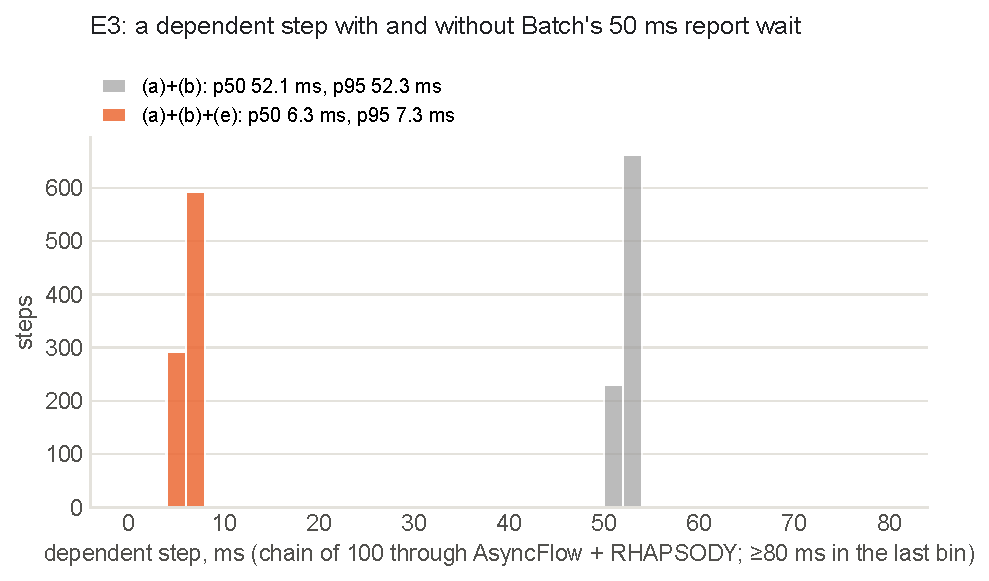
\includegraphics[width=\linewidth]{r4/r4_e3_steps.pdf}
\end{column}
\begin{column}{0.46\textwidth}
\bodysmall
\begin{itemize}
  \item \code{Batch}'s client thread drains completions, then waits up to 50 ms for a submission.
  \item \textbf{(e):} a second thread passes on each completion at once. Off by default; Dragon's 28 \code{Batch} tests pass.
  \item E3's dependent step: \textbf{52.1 to 6.3 ms}, with or without a policy. About 4 ms of it is Dragon's edge.
  \item Throughput and the bulk do not change.
\end{itemize}
\end{column}
\end{columns}
\vfill
{\fontsize{7}{8.4}\selectfont\color{labelgray}julia, 64 CPUs, 32 \code{Batch} workers, capacity 32; Dragon with (a)+(b), with and without (e); median of 3 runs. Trivial tasks: 794--858 against 828--844 per second. E1a's chains: 1.86 to 1.75 s with no policy, 1.62 to 1.59 s with Fair.\par}
\end{frame}

\begin{frame}{One Dragon Process per Task (V1) Against \code{Batch}}
\bodysmall
\begin{center}
  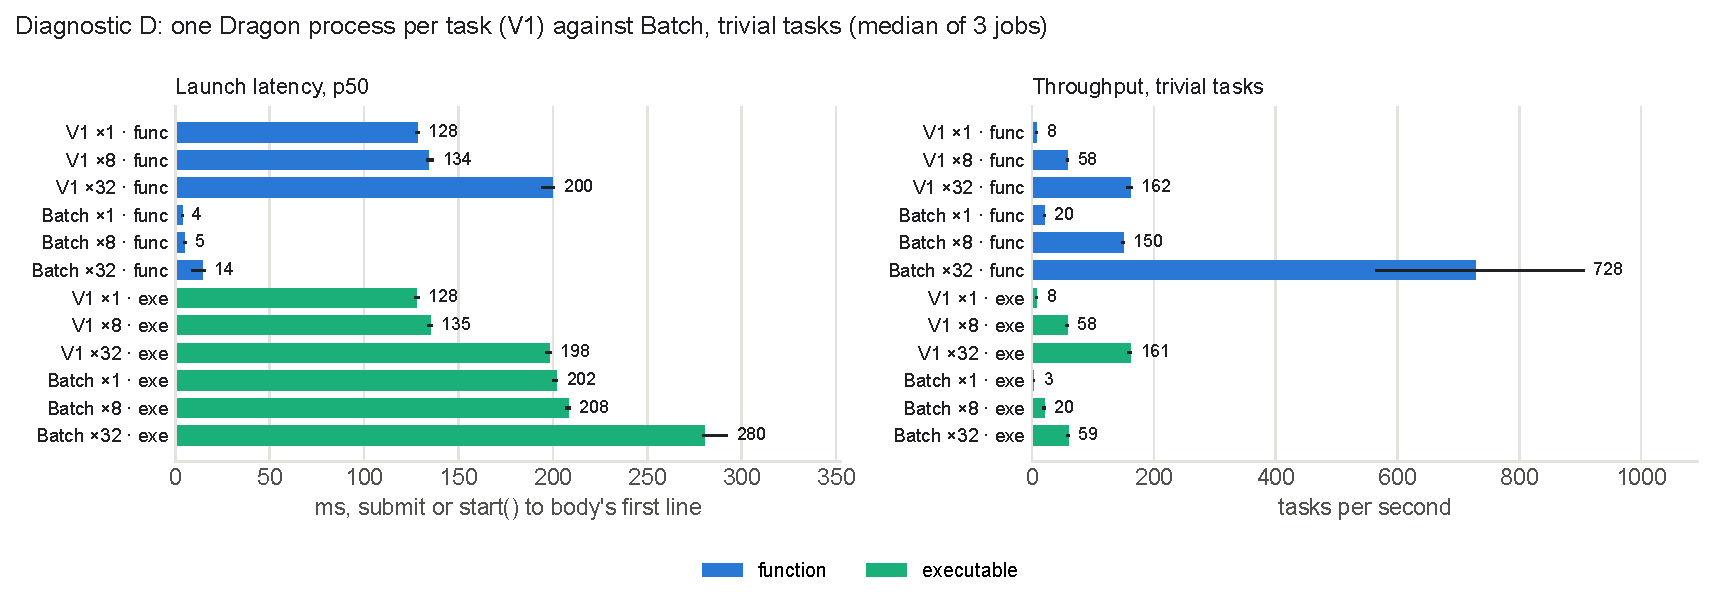
\includegraphics[width=0.8\textwidth]{r3/r3_launch.pdf}
\end{center}
\begin{itemize}
  \item \textbf{V1}, as RHAPSODY did up to 0.4.0: about 130 ms to start a process, 200 ms at 32 in flight.
  \item \textbf{Functions:} \code{Batch} starts them in 4--15 ms, and runs trivial ones 4.5 times faster.
  \item \textbf{Executables:} V1 wins. \code{Batch.process} makes each a one-process job, polled every 0.1 s.
\end{itemize}
\vfill
{\fontsize{7}{8.4}\selectfont\color{labelgray}julia, 64 CPUs; closed loops with 1, 8 and 32 tasks in flight; \code{Batch} with 32 workers and (a)+(b), without (e). With (e), trivial functions reach 1,579 tasks/s at 32 in flight, against 644 in the same check. For 1 s tasks, workers are 84\% busy with V1, 96\% with \code{Batch}.\par}
\end{frame}

\begin{frame}{Subgraphs and a V1 Executor: Not Needed for Speed}
\bodysmall
\begin{columns}[T]
\begin{column}{0.48\textwidth}
\textbf{Submit a chain or a subgraph ahead, so Dragon resolves its edges}
\begin{itemize}
  \item With (e), a dependent step costs 6.3 ms; Dragon's own edge 3--4 ms.
  \item So it saves about 3 ms per edge: it matters only for long chains of millisecond tasks.
  \item Data could stay inside Dragon: a 1 MiB result costs 1.3--1.9 ms per edge today.
  \item If built: hand a slot along an edge. Group chains and fan-ins; stop at a fan-out, or where the resources or the backend change. Dragon still never queues.
\end{itemize}
\end{column}
\begin{column}{0.48\textwidth}
\textbf{Run each task as its own Dragon process, as RHAPSODY's V1 did}
\begin{itemize}
  \item It has no bursts, no 5 ms wait, no \code{Batch} queue and no oversubscription (\#95).
  \item But each task costs about 130 ms to start: \code{Batch} is 4.5 times faster for short functions.
  \item For executables it beats \code{Batch.process} today: 161 against 59 tasks/s.
  \item A hybrid fits: functions through \code{Batch}, executables as one placed Dragon process each. RHAPSODY already runs a placed task that way.
\end{itemize}
\end{column}
\end{columns}
\vfill
\begin{center}
  {\fontsize{11}{13}\selectfont\color{titleink}First, Dragon's two waits: (b) and (e) need no change in AsyncFlow.}
\end{center}
\vfill
\end{frame}

\divider{F. One Dragon Runtime Over Two Nodes}

\begin{frame}{E2 on Two Nodes: The Smaller GPU Overflows}
\bodysmall
\begin{center}
  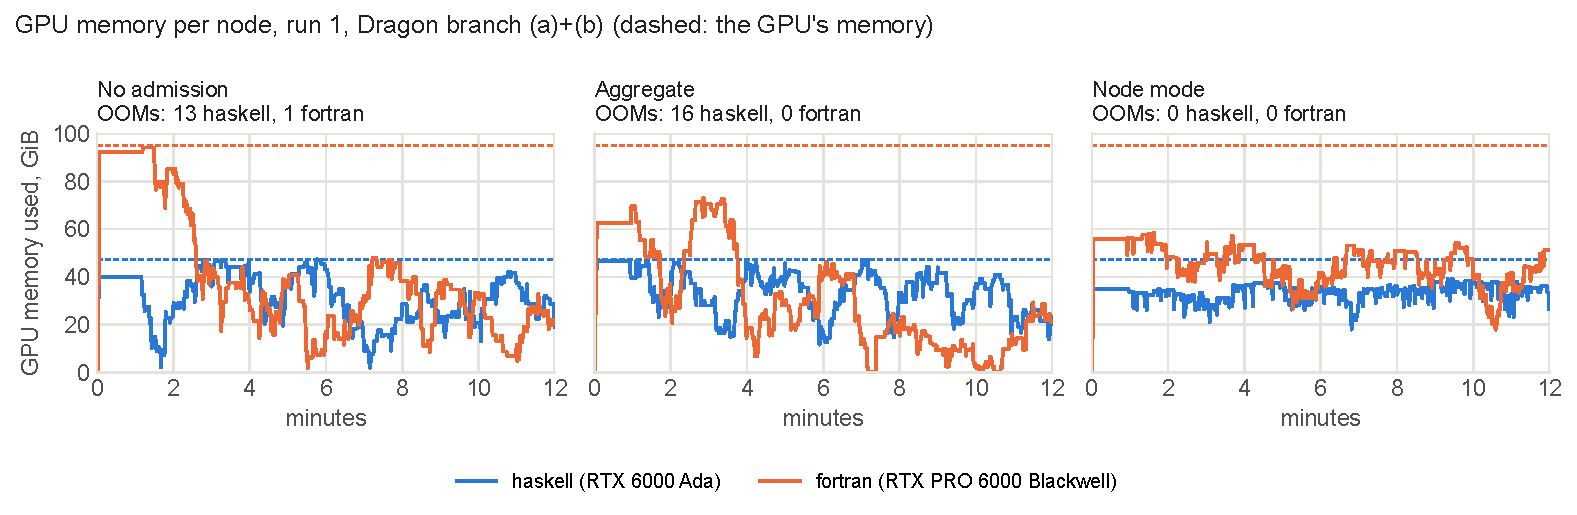
\includegraphics[width=0.85\textwidth]{r3/r3_e2_gpu_memory_branch.pdf}
\end{center}
\begin{itemize}
  \item \code{Batch} sends half the tasks to each node, blind to GPU memory. 178 of 180 OOMs were on haskell.
  \item \textbf{Node mode} puts each task where its memory fits: 0 OOMs, every task where AsyncFlow put it.
\end{itemize}
\vfill
{\fontsize{7}{8.4}\selectfont\color{labelgray}One GPU on each of haskell (RTX 6000 Ada, 47.4 GiB) and fortran (RTX PRO 6000 Blackwell, 95.0 GiB); 24 pipelines. GPU memory $\times$1.5, so that at most 134 GiB is declared against 141.5 GiB: the totals never refuse a task, but haskell's memory binds. 46--56\% of the tasks ran on haskell in every mode.\par}
\end{frame}

\begin{frame}{E2 on Two Nodes: Placement Does More Work}
\begin{lecturetable}{\scriptsize}
\renewcommand{\arraystretch}{1.3}
\begin{tabular}{|B{4.4cm}|L{2.4cm}|L{2.4cm}|L{3.2cm}|}
\hline
\head Admission & CUDA OOMs = pipelines lost, of 24 & Tasks done in 12 min & GPU busy, haskell · fortran \\ \hline
\multicolumn{4}{|l|}{\textit{Stock RHAPSODY + Dragon 0.14.1}} \\ \hline
None (Dragon picks the node) & 16 & 311 & 84\% · 75\% \\ \hline
Aggregate (Dragon picks the node) & 15 & 320 & 81\% · 86\% \\ \hline
Node (AsyncFlow places) & \textbf{0} & \textbf{357} & \textbf{89\% · 92\%} \\ \hline
\multicolumn{4}{|l|}{\textit{Dragon branch, (a)+(b)}} \\ \hline
None (Dragon picks the node) & 14 & 326 & 85\% · 81\% \\ \hline
Aggregate (Dragon picks the node) & 16 & 322 & 76\% · 82\% \\ \hline
Node (AsyncFlow places) & \textbf{0} & \textbf{370} & \textbf{93\% · 97\%} \\ \hline
\end{tabular}
\end{lecturetable}
\vspace{4pt}
\bodysmall
\begin{itemize}
  \item Node mode: 0 OOMs in 6 runs, and 12--15\% more tasks than the other modes. On one node, admission bought no throughput; here it does.
  \item Aggregate is no better than none: the OOMs come from the node choice, not the totals.
\end{itemize}
\vfill
{\fontsize{7}{8.4}\selectfont\color{labelgray}A heterogeneous Slurm job, as haskell and fortran share no partition: 28 CPUs, 1 GPU and 64 GiB on each, 14 \code{Batch} workers per node. A wrapper of Dragon's \code{srun} calls lets one runtime span both. 12-minute window; median of 3 runs.\par}
\end{frame}

\begin{frame}{Two Nodes: The Policies Hold, Throughput Drops}
\begin{lecturetable}{\scriptsize}
\renewcommand{\arraystretch}{1.25}
\begin{tabular}{|B{4.6cm}|L{1.9cm}|L{1.9cm}|L{1.9cm}|L{1.9cm}|}
\hline
\head & \multicolumn{2}{l|}{\textbf{One node}} & \multicolumn{2}{l|}{\textbf{Two nodes}} \\ \hline
\head Measure & No policy & Policy & No policy & Policy \\ \hline
\multicolumn{5}{|l|}{\textit{Dragon branch, (a)+(b)}} \\ \hline
E3: trivial tasks/s, Fair & 836 & 853 & 311 & 354 \\ \hline
E3: trivial tasks/s, Lineage & 836 & 837 & 311 & 333 \\ \hline
E1a: chain p50, Fair & 1.86 s & 1.59 s & 2.07 s & 2.17 s \\ \hline
E1a: bulk makespan, Fair & 98.4 s & 99.1 s & 100.8 s & 107.3 s \\ \hline
E1b: mean completion, Lineage & 26.4 s & \textbf{18.4 s} & 26.3 s & \textbf{19.7 s} \\ \hline
\multicolumn{5}{|l|}{\textit{Stock Dragon + the no-change patch}} \\ \hline
E1a: chain p50, Fair & 13.1 s & 1.65 s & 16.8 s & 4.65 s \\ \hline
\end{tabular}
\end{lecturetable}
\vspace{2pt}
\bodysmall
\begin{itemize}
  \item Per-task reports hold across nodes; capacity 32 still matches no policy.
  \item Fair's chains slow from 1.6 to 2.2 s: each refill goes through the slower two-node runtime.
  \item Two nodes cut trivial-task throughput by 58--63\%, even for raw \code{Batch} on one of them. Bridges-2 shows why: the runtime spanning nodes costs it (section G).
\end{itemize}
\vfill
{\fontsize{7}{8.4}\selectfont\color{labelgray}Two nodes: haskell and julia, 32 CPUs each, 16 \code{Batch} workers per node. One node: julia, 64 CPUs, 32 workers, earlier the same day. Capacity 32; median of 3 runs; before switch (e). \code{Batch} puts a task compiled alone on a random node; a dependent step costs the same on either.\par}
\end{frame}

\divider{G. Two and Four Nodes on Bridges-2}

\begin{frame}{Bridges-2: The Policies Hold on Four Nodes}
\centerline{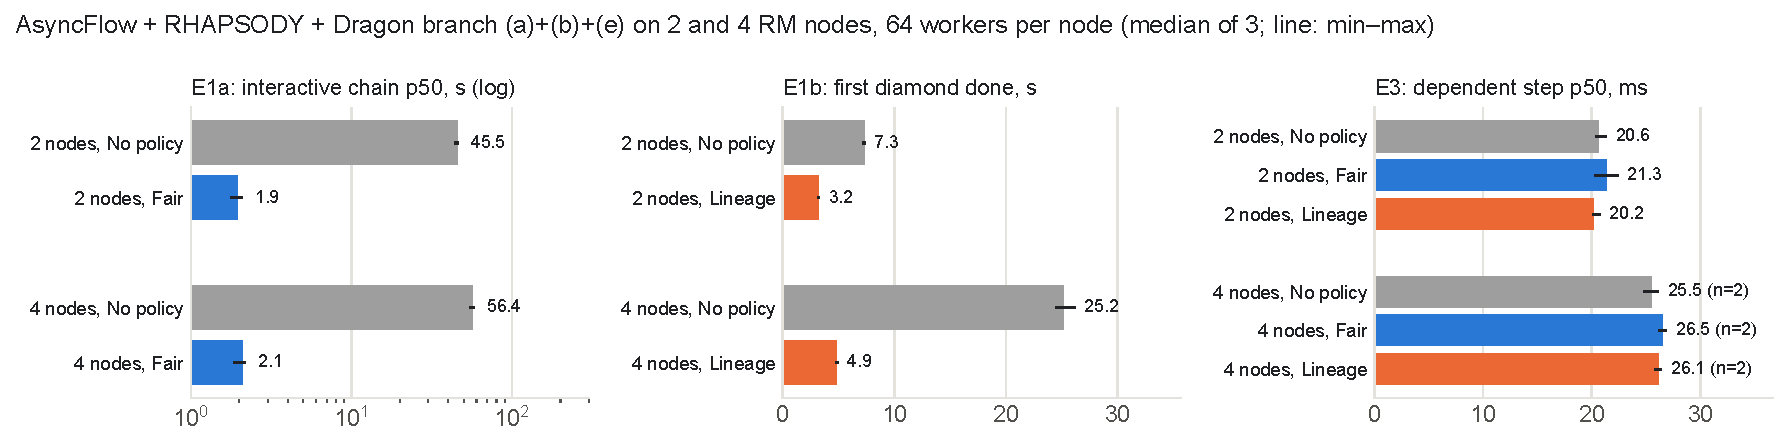
\includegraphics[width=0.88\linewidth]{b2/charts/b2_af.pdf}}
\bodysmall
\begin{itemize}
  \item Fair keeps chains at about 2 s beside growing bulk work; the bulk takes 3--4\% longer.
  \item Lineage: the first diamond 2--5 times sooner, one pool's worth open (256, not 1,592); makespan +4\% on two nodes, +15\% on four.
  \item No cost per dependent step at the median; on four nodes the p95 falls from 177 to 42--48 ms.
  \item No policy: the workers, not the nodes, lengthen chains: 1.8, 21 and 44 s at 32, 64 and 128 on one node; 46 s at 128 on two, 56 s at 256 on four.
\end{itemize}
\vfill
{\fontsize{7}{8.4}\selectfont\color{labelgray}PSC Bridges-2 RM, 128 cores and 64 \code{Batch} workers per node (one-node follow-ups: 32--128), capacity = pool; Dragon branch (a)+(b)+(e), TCP over InfiniBand; workloads per 32 workers as on rust. Median of 3 runs (E3 on four nodes: 2; one hung in Dragon).\par}
\end{frame}

\begin{frame}{Bridges-2: A Multi-Node Runtime Costs Throughput}
\centerline{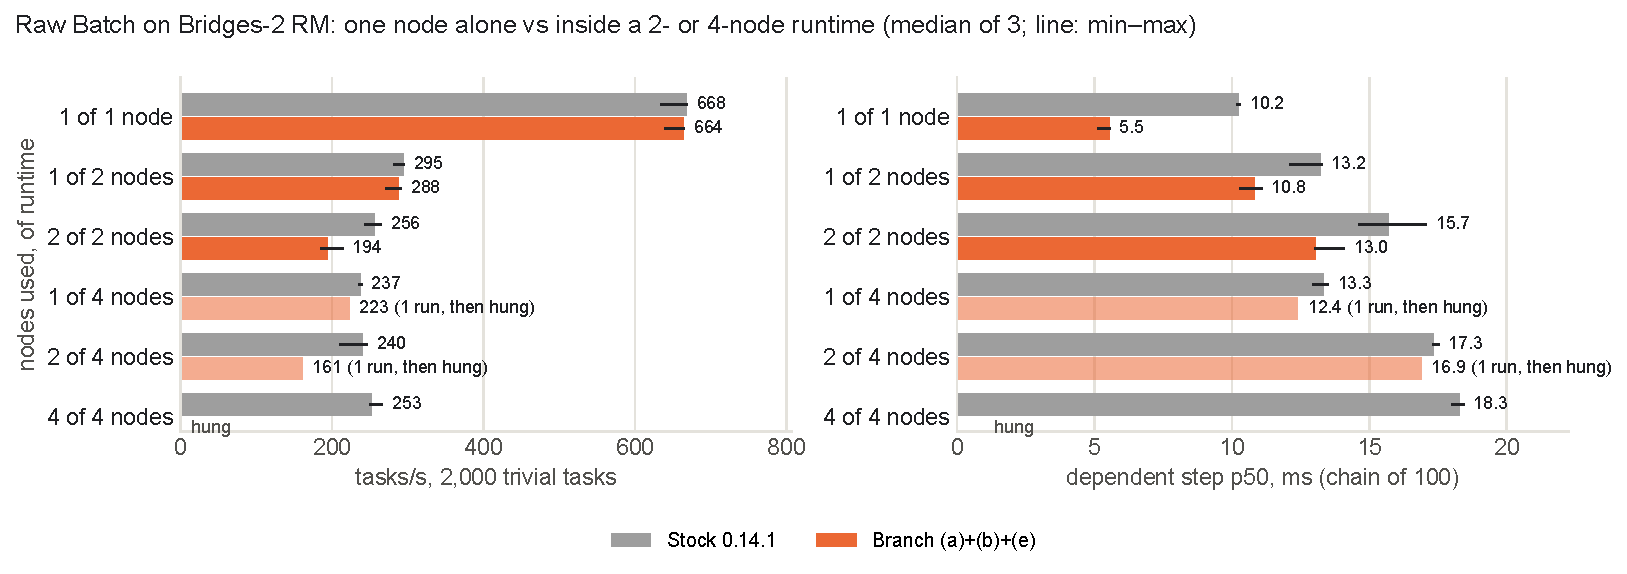
\includegraphics[width=0.64\linewidth]{b2/charts/b2_raw_batch.pdf}}
\bodysmall
\begin{itemize}
  \item One node does 668 trivial tasks/s alone, 295 inside a two-node runtime, 237 inside a four-node one; using more of its nodes changes little.
  \item So rust's two-node loss is \code{Batch} in a multi-node runtime, not AsyncFlow, RHAPSODY or task placement.
  \item The branch halves the one-node step (10.2 to 5.5 ms) but costs throughput across nodes (256 to 194 tasks/s); it hung on four.
\end{itemize}
\vfill
{\fontsize{7}{8.4}\selectfont\color{labelgray}Raw \code{Batch}: 2,000 trivial tasks and a chain of 100, in 1-, 2- and 4-node runtimes on the same 4 nodes; dragonhpc 0.14.1, 64 workers per node. Median of 3 runs.\par}
\end{frame}

\begin{frame}{Bridges-2: \#95 Fixed Again; a GPU Density Limit}
\bodysmall
\begin{lecturetable}{\footnotesize}
\begin{tabular}{|B{5.4cm}|L{2.6cm}|L{2.6cm}|L{2.6cm}|}
\hline
\head RM-shared job & One trivial task & \#95's workflow & Shutdown \\ \hline
4 cores, RHAPSODY 0.6.0 (64 workers) & 15.2 s & 21.0 s & 31.8 s \\ \hline
4 cores, pool cap (2 workers) & 0.78 s & 0.56 s & 1.6 s \\ \hline
16 cores, RHAPSODY 0.6.0 (64 workers) & 2.6 s & 8.0 s & 2.8 s \\ \hline
16 cores, pool cap (8 workers) & 0.37 s & 0.50 s & 1.3 s \\ \hline
\end{tabular}
\end{lecturetable}
\vspace{4pt}
\begin{itemize}
  \item \textbf{GPU nodes:} with 48 \code{Batch} workers on 20 cores (32 pipelines on 4 V100s), Dragon 0.14.1 stalled or failed to launch tasks in 4 of 4 runs. Up to 32 workers ran clean, at 8 tasks per GPU, with no CUDA OOM.
  \item So the limit lies between 1.6 and 2.4 workers per core. A 40-core, 8-GPU node should run IMPRESS's 8 per GPU with 64 workers; E2 is not run yet.
\end{itemize}
\vfill
{\fontsize{7}{8.4}\selectfont\color{labelgray}Stock dragonhpc 0.14.1; median of 2 runs per row; the 4-core 0.6.0 runs shared their node with other jobs. GPU tests: GPU-shared, V100-SXM2-32GB, 5 cores per GPU. 850 RM and 3.9 GPU SU in all.\par}
\end{frame}

\divider{H. Two and Four Nodes on Perlmutter}

\begin{frame}{Perlmutter: The Policies Hold on Both Backends}
\centerline{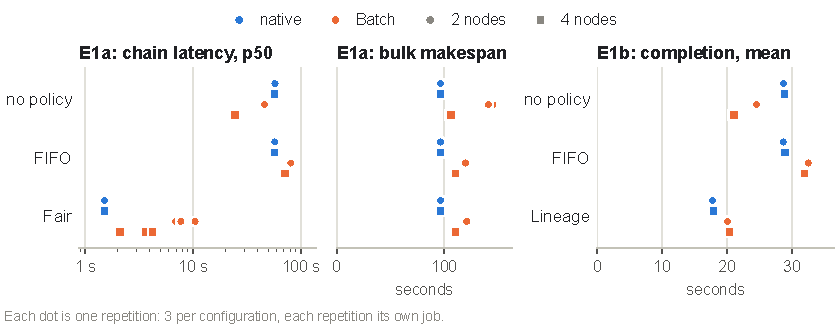
\includegraphics[width=0.60\linewidth]{pm/charts/pm_policy_order.pdf}}
\bodysmall
\begin{itemize}
  \item Fair: chains 57--58 to 1.5 s on native, 25--46 to 2.1--10.5 s on \code{Batch}. The bulk: unchanged on native; on \code{Batch}, 3--5\% slower to 15\% faster.
  \item Lineage: diamonds finish sooner: native 28.7 to 17.8 s; \code{Batch} 24.5 to 20.1 s (two nodes), 20.9 to 20.1 s (four).
  \item FIFO adds nothing: native's queue is already first in, first out; on \code{Batch} it lengthens chains to 70--81 s.
\end{itemize}
\vfill
{\fontsize{7}{8.4}\selectfont\color{labelgray}NERSC Perlmutter CPU nodes (128 cores), stock dragonhpc 0.15.0 over HSTA. Native: a RHAPSODY backend on Dragon's native API, a pool of placed workers. 64 workers per node, capacity = pool; workloads per 32 workers as on rust. 3 runs each, each its own job.\par}
\end{frame}

\begin{frame}{Perlmutter: The Backend, Not the Policy, Sets the Cost}
\centerline{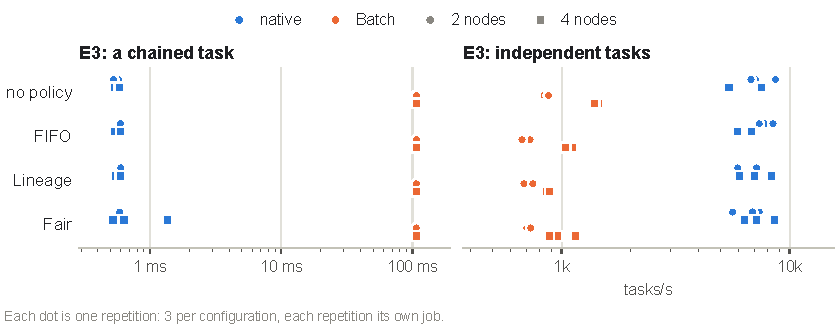
\includegraphics[width=0.62\linewidth]{pm/charts/pm_policy_cost.pdf}}
\bodysmall
\begin{itemize}
  \item A dependent step: 0.5--0.6 ms on native, 107 ms on \code{Batch}, with or without a policy. 0.15.0's \code{Batch} manager waits 50 ms per loop (57 ms on rust's 0.14.1).
  \item Trivial tasks: native 5,400--8,700 tasks/s under every policy. On \code{Batch}, as on rust, a capacity costs throughput: 14--23\% on two nodes, 20--36\% on four.
  \item So native keeps the policies' gains and removes the cost of a capacity.
\end{itemize}
\vfill
{\fontsize{7}{8.4}\selectfont\color{labelgray}Same runs. A dependent step: a chain of 100 trivial tasks, each taking the previous result. Trivial tasks: 2,000 submitted at once, from the first submission to the last result.\par}
\end{frame}

\divider{I. Status}

\begin{frame}{Cooperation Needs Prompt Reports, Not Priorities}
\begin{center}
  \begin{tikzpicture}
    \node[bluebox, text width=13.4cm, font=\fontsize{9.5}{11.4}\selectfont, inner sep=5pt]
      {Dragon reports each task at once when it ends. AsyncFlow, which knows the workflow, orders tasks by admission, keeps at most a pool's worth inside Dragon, and places GPU tasks where they fit.};
  \end{tikzpicture}
\end{center}
\begin{lecturetable}{\scriptsize}
\renewcommand{\arraystretch}{1.2}
\begin{tabular}{|B{5.0cm}|L{6.4cm}|L{2.2cm}|}
\hline
\head What we ask Dragon & Evidence on rust & Local branch \\ \hline
Report each task when it ends & Workers 96\% busy, not 59--67\%; chains 26.9 to 1.9 s & Yes, (b) \\ \hline
Pass each completion to the client at once & A dependent step: 52 to 6.3 ms & Yes, (e) \\ \hline
Let a client turn off the 5 ms wait & Fair at capacity 32: 533 to 853 tasks/s & Yes, (a) \\ \hline
Break ties by number, not by task id as text & \code{"1-1031"} runs before \code{"1-532"} & No \\ \hline
Size \code{Batch} from the job's CPUs & Issue \#95: one task on 4 CPUs, 111 to 0.3 s & Yes \\ \hline
A light path for a single-process task & \code{Batch.process} 59 tasks/s; a process per task 161 & No \\ \hline
Pick nodes by free GPU memory; say where tasks ran & Two GPUs, totals fit: 13--17 OOMs per run on the smaller & No \\ \hline
Report each task's peak memory & Learned memory for \code{ResourcePolicy} & Yes \\ \hline
\end{tabular}
\end{lecturetable}
\vfill
\bodysmall
Not needed: a priority per task; it helps only above the pool size, where Fair's priorities go stale. The branch is not a release: it hung twice on four Bridges-2 nodes.
\vfill
\end{frame}

\begin{frame}{What Is Proven, and What Is Not Yet}
\bodysmall
\begin{columns}[T]
\begin{column}{0.48\textwidth}
\textbf{Measured}
\begin{itemize}
  \item Tickless engine on Python 3.9--3.14; Dragon cancellations in 0.1--0.3 ms.
  \item The policies' behaviour, in 61 unit tests.
  \item Real Dragon: Fair cut chains 4--11 times; Lineage finished workflows 25--30\% sooner.
  \item Four nodes, Fair: chains 56 to 2.1 s (Bridges-2), 58 to 1.5 s (Perlmutter, native).
  \item Real GPUs: no OOM in node mode, on one node or two; on two, 12--15\% more work.
  \item No measurable latency cost per task.
  \item Dragon: \#95, the bursts and the 50 ms wait, fixed locally. A dependent step: 57 to 6.3 ms.
  \item A capacity above the pool: no gain.
\end{itemize}
\end{column}
\begin{column}{0.48\textwidth}
\textbf{Not yet}
\begin{itemize}
  \item IMPRESS on 8 real nodes (two so far).
  \item E2 on more GPUs; on Bridges-2, Dragon 0.14.1 stalls at 2.4 workers per core.
  \item Learned memory on Dragon (a local branch reports peaks).
  \item Per-task reports and the completion wake-up in a Dragon release.
  \item Whether Bridges-2's 55--65\% multi-node loss is \code{Batch}'s results store, as on rust.
  \item Stock Dragon's 10 ms floor per dependent step; where the last 2--3 ms of the 6.3 ms step go.
\end{itemize}
\end{column}
\end{columns}
\end{frame}

\begin{frame}{Next Steps}
\begin{itemize}
  \item Merge in order: \#100, \#110 (which replaces \#91), then ordering policies, then resource-aware admission.
  \item RHAPSODY: \#105 (cancellations on the event loop) is merged; next, the pool cap and the placement PR. Until Dragon reports each task, compile each task alone, with a cleaner mechanism than the patch. Try executables as one Dragon process each.
  \item AsyncFlow: keep the capacity at the pool size; priorities stay an experimental option. No submitting ahead for now: with (e), it would save about 3 ms per step.
  \item Dragon: show the team the diagnostics, then the asks, per-task reports (b) and the completion wake-up (e) first.
  \item On Bridges-2: E2 at 8 tasks per GPU with 1.6 workers per core; how often the branch hangs on four nodes. On rust: E2 on four GPUs; learned memory. Then IMPRESS on 8 Delta nodes with node mode.
\end{itemize}
\end{frame}

\end{document}
